\documentclass[tikz,border=3pt]{standalone}
\usepackage[T1]{fontenc}
\usepackage{lmodern}
\usetikzlibrary{arrows.meta,positioning,fit,backgrounds,calc}
\definecolor{preblue}{RGB}{35,87,137}
\definecolor{runtimeorange}{RGB}{181,82,36}
\begin{document}
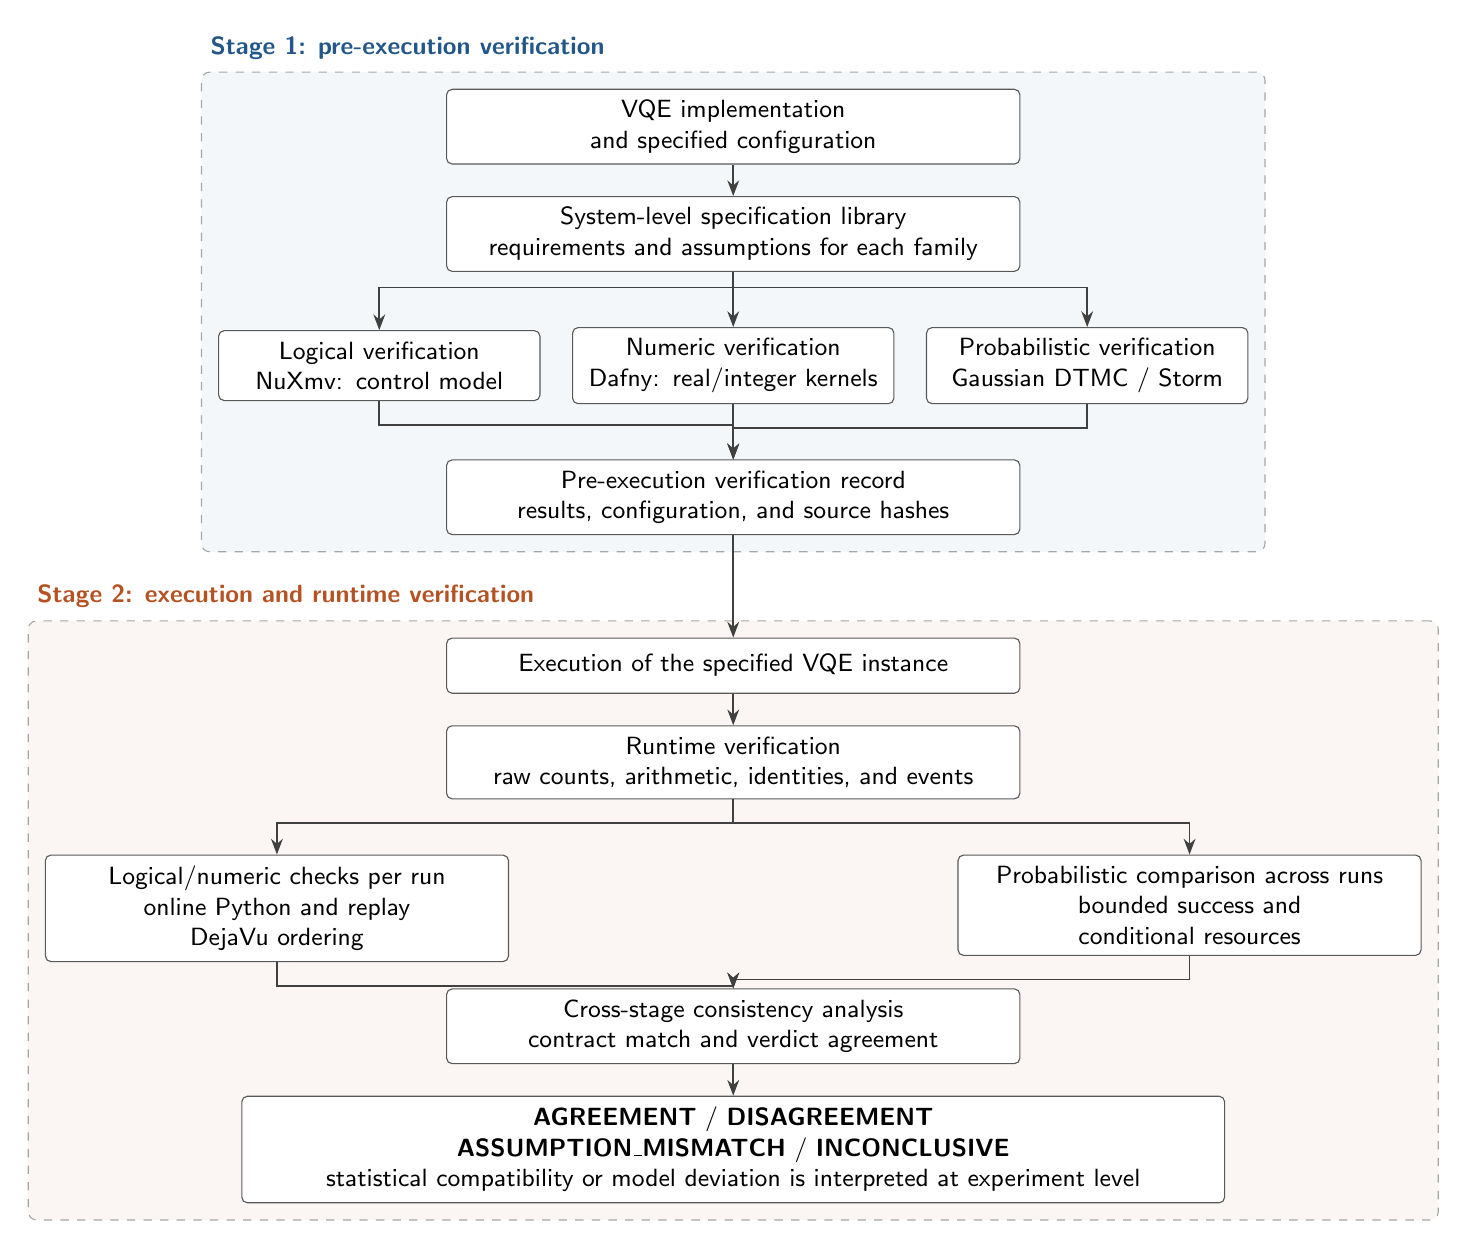
\begin{tikzpicture}[font=\sffamily\small,
 box/.style={draw=black!65,rounded corners=2pt,fill=white,align=center,minimum height=7mm,inner sep=4pt},
 arr/.style={-{Stealth[length=2mm]},semithick,draw=black!75},
 stage/.style={rounded corners=3pt,draw=black!35,dashed,inner sep=6pt}]
\node[box,text width=7cm] (vqe) at (0,0) {VQE implementation\\and specified configuration};
\node[box,text width=7cm,below=4mm of vqe] (library) {System-level specification library\\requirements and assumptions for each family};
\node[box,text width=3.8cm,below=7mm of library] (numeric) {Numeric verification\\Dafny: real/integer kernels};
\node[box,text width=3.8cm,left=4mm of numeric] (logical) {Logical verification\\NuXmv: control model};
\node[box,text width=3.8cm,right=4mm of numeric] (prob) {Probabilistic verification\\Gaussian DTMC / Storm};
\node[box,text width=7cm,below=7mm of numeric] (record) {Pre-execution verification record\\results, configuration, and source hashes};
\draw[arr] (vqe)--(library);
\foreach \n in {logical,numeric,prob} {\draw[arr] (library.south)--++(0,-2mm)-|(\n.north); \draw[arr] (\n.south)--++(0,-3mm)-|(record.north);}
\node[box,text width=7cm,below=13mm of record] (execution) {Execution of the specified VQE instance};
\node[box,text width=7cm,below=4mm of execution] (observations) {Runtime verification\\raw counts, arithmetic, identities, and events};
\node[box,text width=5.6cm,below left=7mm and -8mm of observations] (det) {Logical/numeric checks per run\\online Python and replay\\DejaVu ordering};
\node[box,text width=5.6cm,below right=7mm and -8mm of observations] (emp) {Probabilistic comparison across runs\\bounded success and conditional resources};
\node[box,text width=7cm,below=24mm of observations] (analysis) {Cross-stage consistency analysis\\contract match and verdict agreement};
\node[box,text width=12.2cm,below=4mm of analysis] (verdict) {\textbf{AGREEMENT} / \textbf{DISAGREEMENT}\\\textbf{ASSUMPTION\_MISMATCH} / \textbf{INCONCLUSIVE}\\statistical compatibility or model deviation is interpreted at experiment level};
\draw[arr] (record)--(execution); \draw[arr] (execution)--(observations);
\foreach \n in {det,emp} {\draw[arr] (observations.south)--++(0,-3mm)-|(\n.north); \draw[arr] (\n.south)--++(0,-3mm)-|(analysis.north);}
\draw[arr] (analysis)--(verdict);
\begin{scope}[on background layer]
\node[stage,fill=preblue!5,fit=(vqe)(logical)(prob)(record)] (stageone) {};
\node[stage,fill=runtimeorange!5,fit=(execution)(det)(emp)(analysis)(verdict)] (stagetwo) {};
\end{scope}
\node[font=\sffamily\bfseries\small,anchor=west,text=preblue] at ($(stageone.north west)+(0,3mm)$) {Stage 1: pre-execution verification};
\node[font=\sffamily\bfseries\small,anchor=west,text=runtimeorange] at ($(stagetwo.north west)+(0,3mm)$) {Stage 2: execution and runtime verification};
\end{tikzpicture}
\end{document}
